\subsection{Platform Initialization \gls{pi} Boot Sequence}
Platform Initialization \gls{pi} compliant system firmware has to support the six phases: 
\begin{enumerate}
	\item \say{Security (\gls{sec})} Phase
	\item \say{Pre-efi Initialization (\gls{pei})} Phase
	\item \say{Driver Execution Environment (\gls{dxe})} Phase
	\item \say{Boot device selection (\gls{bds})} Phase
	\item \say{Run time (RT)} services 
	\item \say{After Life (AL)} of system. 
\end{enumerate}
Figure \ref{fig:design-pi-boot-phases} describes the phases and transition in detail.

\begin{figure}[!htbp]
	\centering
	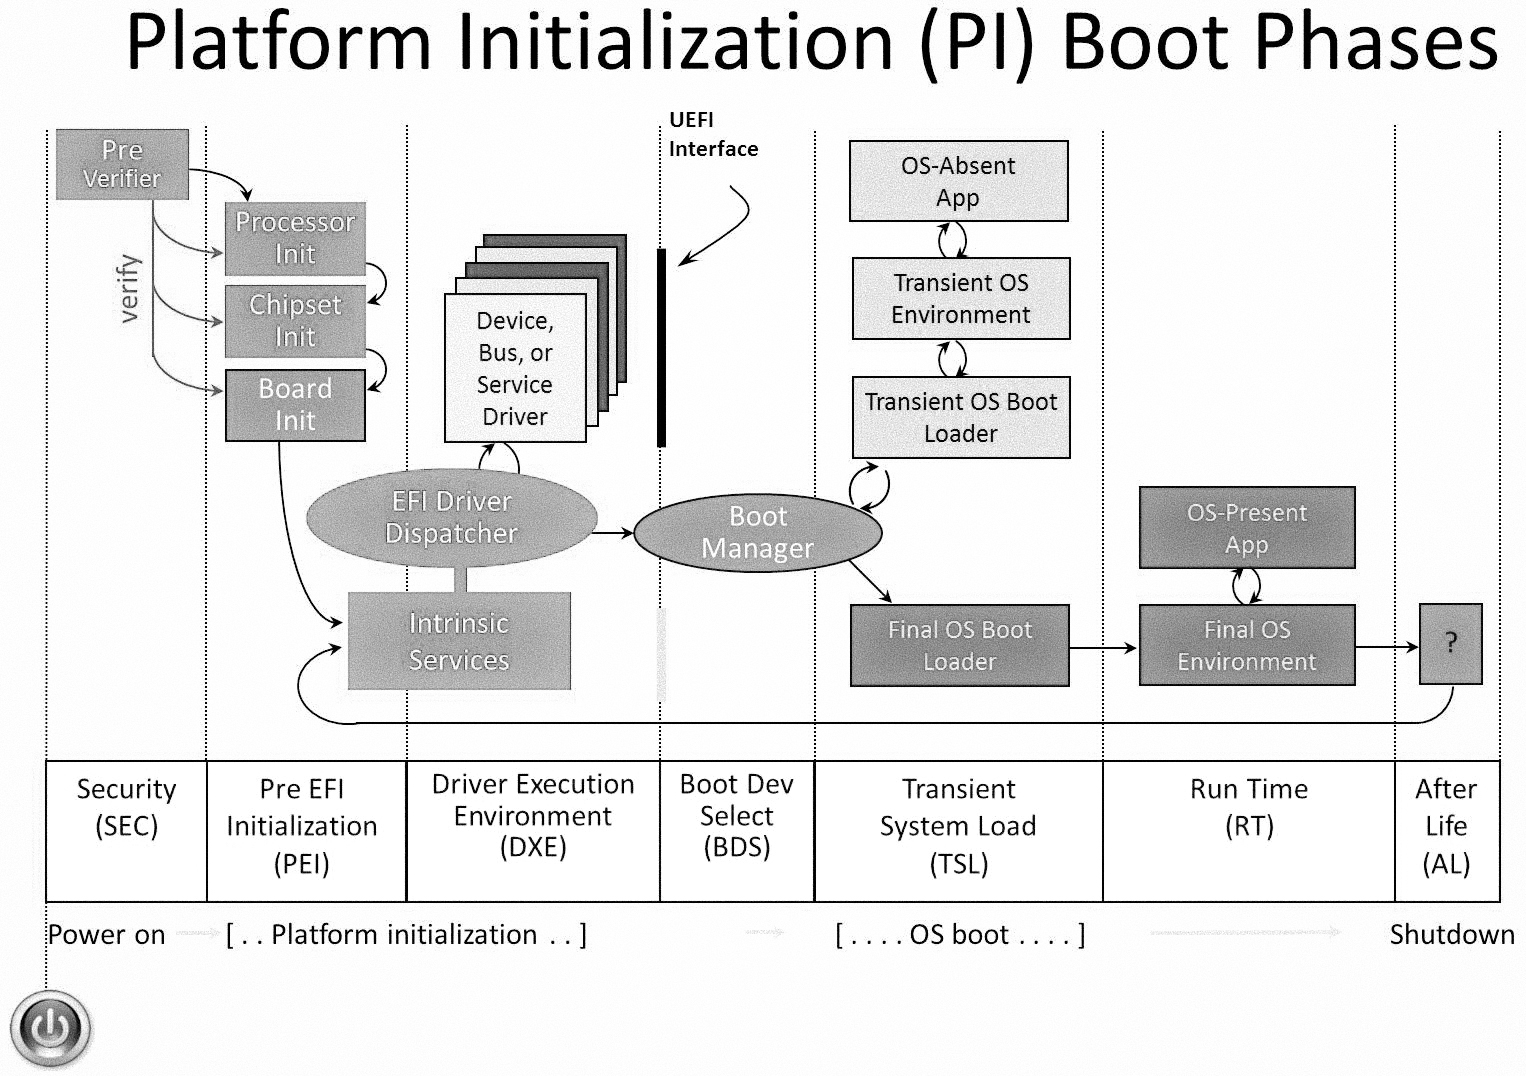
\includegraphics[width=\linewidth]{PI_Boot_Phases}
	\caption{\gls{pi} Boot Phases}\label{fig:design-pi-boot-phases}
\end{figure}

\subsection{Security (\gls{sec})}
\say{Security (SEC)} phase is the initial phase through which the boot flow begins. This phase is responsible for the following:
\begin{itemize}
	\item Handling restart events of every platform
	\item Creation of a temporary memory stash
	\item Bringing the trust root in the system
	\item Transit handoff content to next phase - the \say{PEI Foundation}
\end{itemize}

Figure \ref{fig:sec-phase} portrays the Flow of the DXE phase.

\begin{figure}[!htbp]
	\centering
	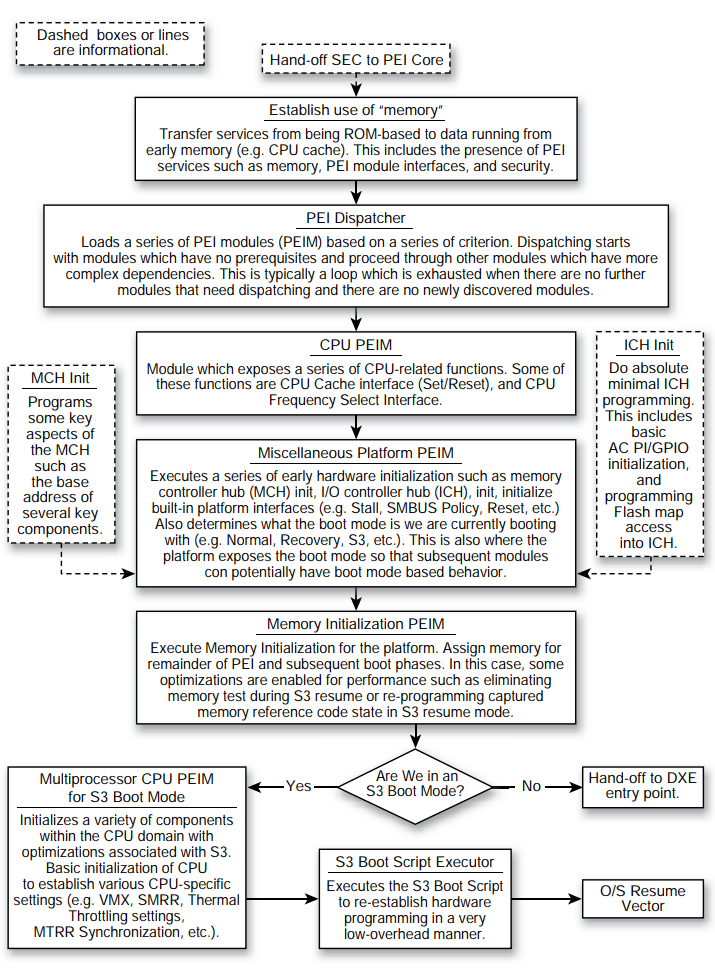
\includegraphics[width=\linewidth]{design/pei-phase}
	\caption{SEC Phase}\label{fig:sec-phase}
\end{figure}

The security section may have the modules with source code scripted in assembly language. Hence, some \gls{edk2} module development environment (MDE) modules can consist of assembly code. During Occurrence of this, both Windows and GCC versions of assembly language code are served in different files.

\subsection{Pre-EFI Initialization (\gls{pei})}
\say{Pre-EFI Initialization (PEI)} phase represented within the PI Architecture specifications brought up quite betimes in the period of boot. Especially, after about preliminary processing of the Security (SEC) phase, any system restart event will bring up the PEI phase.

The PEI phase is designed to be developed in many parts and consists of:
\begin{itemize}
	\item PEI Foundation (core code)
	\item Pre-EFI Initialization Modules (specialized plug-ins)
\end{itemize}

The PEI phase at first operates along the platform in a developing stage, holding only resources on processor, such as the cache for maintaining call stack and dispatching the \say{Pre-EFI Initialization Modules (PEIMs)}.

Figure \ref{fig:pei-phase} portrays the Flow of the DXE phase.

\begin{figure}[!htbp]
	\centering
	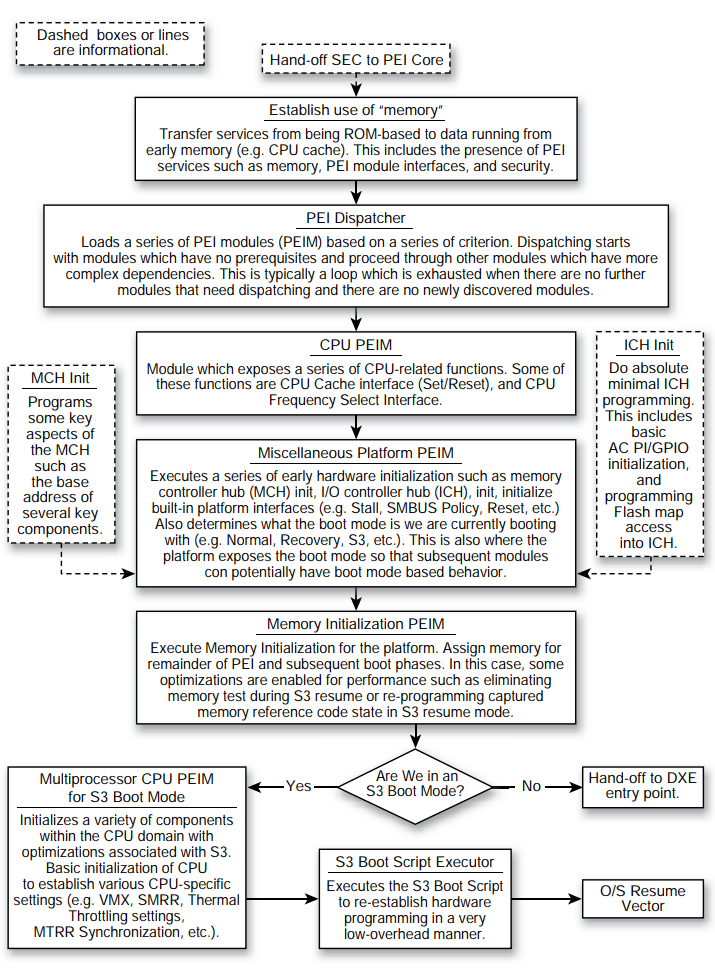
\includegraphics[width=\linewidth]{design/pei-phase}
	\caption{PEI Phase}\label{fig:pei-phase}
\end{figure}

The PEI phase can not presume the convenience of amount of main memory (RAM) as DXE and hence PEI phase support is limited to:
\begin{itemize}
	\item Locates and validates PEIMs
	\item Dispatches of PEIMs
	\item Facilitates commuting of PEIMs
	\item Provides handoff information content to later phases
\end{itemize}

These PEIMs can be considered for accountable for:
\begin{itemize}
	\item Initializing few permanent memory complement
	\item Characterizing the main memory in \say{Hand-Off Blocks (HOBs)}
	\item Characterizing locations of the firmware volume in HOBs
	\item Transit the control flow into next phase - the \say{Driver Execution Environment (DXE)} phase
\end{itemize}

Figure \ref{fig:design-pei-operation-diagram} shows a diagram describes the action carried out during the PEI phase

\begin{figure}[h]
	\centering
	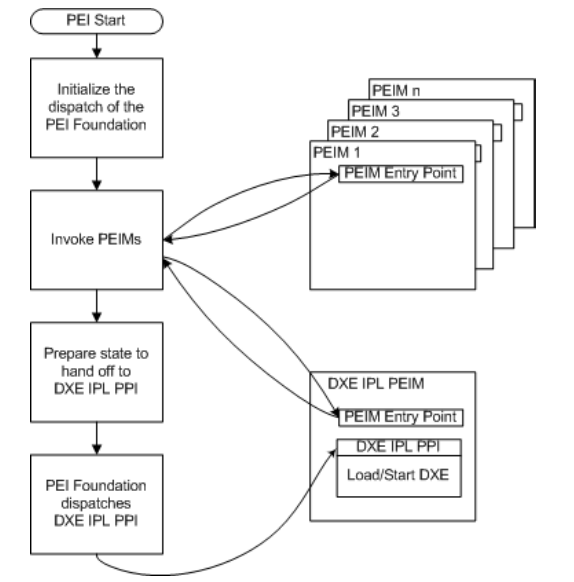
\includegraphics[width=0.8\linewidth]{design/pei-operation-diagram}
	\caption{Diagram of PI Operations}\label{fig:design-pei-operation-diagram}
\end{figure}

\subsubsection{PEI Services}
\say{PEI Foundation} institutes a system table for the PEI Services named as \say{PEI Services Table} which is viewable to every \gls{pei} Modules (PEIMs) exists on the system. A PEI Service could be defined as a method, command or some other potentiality manifested by the \say{PEI Foundation} when the requirements of that service initialization are fulfilled. As the PEI phase having no permanent memory accessible until almost the end of life of the phase, all the various types of services constructed during this phase (\say{PEI phase}) cannot be as enrich as those constructed during later phases. A pointer referenced to PEI Services Table is sent to the entry point of each and every PEIM and also within part of each \say{PEIM-to-PEIM Interface (PPI)} because the location of PEI Foundation and its temporary storage memory is unknown at the time of build. 

\subsubsection{PEI Foundation}
The Phase PEI Foundation carries out following activity:
\begin{itemize}
	\item Dispatching of \say{Pre-EFI initialization modules (PEIMs)}
	\item Maintaining and managing the boot mode
	\item Initialization of permanent main memory
	\item Conjure the DXE loader 
\end{itemize}
The PEI Foundation developed to be portable among all the various platforms architecture of a specified instruction-set. i.e. A binary for \say{IA-32} (32-bit Intel architecture) works across all Pentium processors and similarly \say{Itanium® processor family} works on all the Itanium processors.

Irrespective of the processor's micro architecture, the set of service routines uncovered by the PEI Foundation has to be the same. This consistent layered area over the PEI Foundation allows PEIMs to be developed by the \say{C programming language} and also be compiled across any micro architecture.

The PEI Foundation responsible in providing the service classes listed in Figure \ref{fig:pei-foundation-service-class}
\begin{figure}[!htbp]
	\centering
	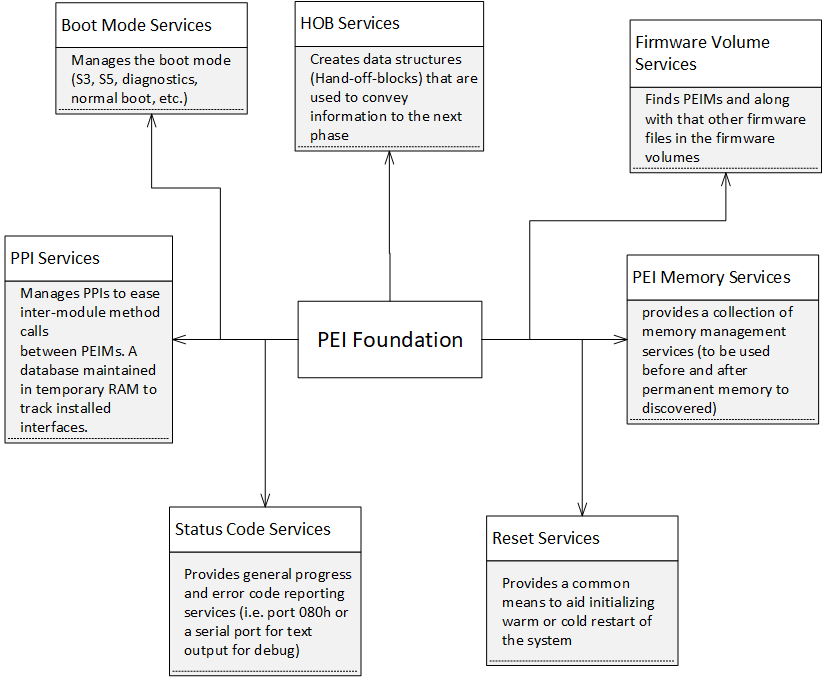
\includegraphics[width=\linewidth]{design/pei-foundation-service-class}
	\caption{Services provided by PEI Foundation classes}\label{fig:pei-foundation-service-class}
\end{figure}

\subsubsection{PEI Dispatcher}
The implementation of a state machine in PEI Foundation is known as the PEI Dispatcher. It evaluates the dependency expressions (DEPEX) in \say{Pre-EFI initialization modules (PEIMs)} that are lying in the \gls{fv}s being analyzed.

Dependency expressions (DEPEX) are coherent alliance of \say{PEIM-to-PEIM Interfaces (PPIs)}. These expressions distinguish the PPIs that has to be available for use before invoked by a given PEIM. The PEI Dispatcher references the PPI database in the PEI Foundation to conclude which PPIs have to be installed and evaluate the dependency expression for the PEIM. If PPI has already been installed then dependency expression (DEPEX) will evaluate the result to \verb|TRUE| which informs PEI Dispatcher that it can execute PEIM. At this very stage, the PEI Foundation handovers control flow to the PEIM with DEPEX result evaluated to \verb|TRUE|. 

The PEI Dispatcher will exit when it has examined and evaluated the results of all the PEIMs in all of the uncovered firmware volumes and none of the PEIMs can be dispatched (such as the \gls{depex} do not evaluate from \verb|FALSE| to \verb|TRUE| and vice-versa). At this stage, the PEI Dispatcher can not make call to any extra PEIMs. Control flow is than taken back by the PEI Foundation from the PEI Dispatcher and call to the \verb|DXE IPL PPI| is made to navigate control flow to the \say{DXE phase} of execution.

\subsection{Driver eXecution Environment (\gls{dxe})}
Before the \say{DXE phase} the \say{Pre-EFI Initialization (PEI)} phase is held liable for initializing the permanent memory on the system platform. Hence, DXE phase could be loaded and executed in the permanent memory. At the very end of the PEI phase, state of the system is handed over to the DXE phase via utilizing the Hand-Off Blocks (HOBs). 

Figure \ref{fig:dxe-phase} portrays the Flow of the DXE phase.

\begin{figure}[!htbp]
	\centering
	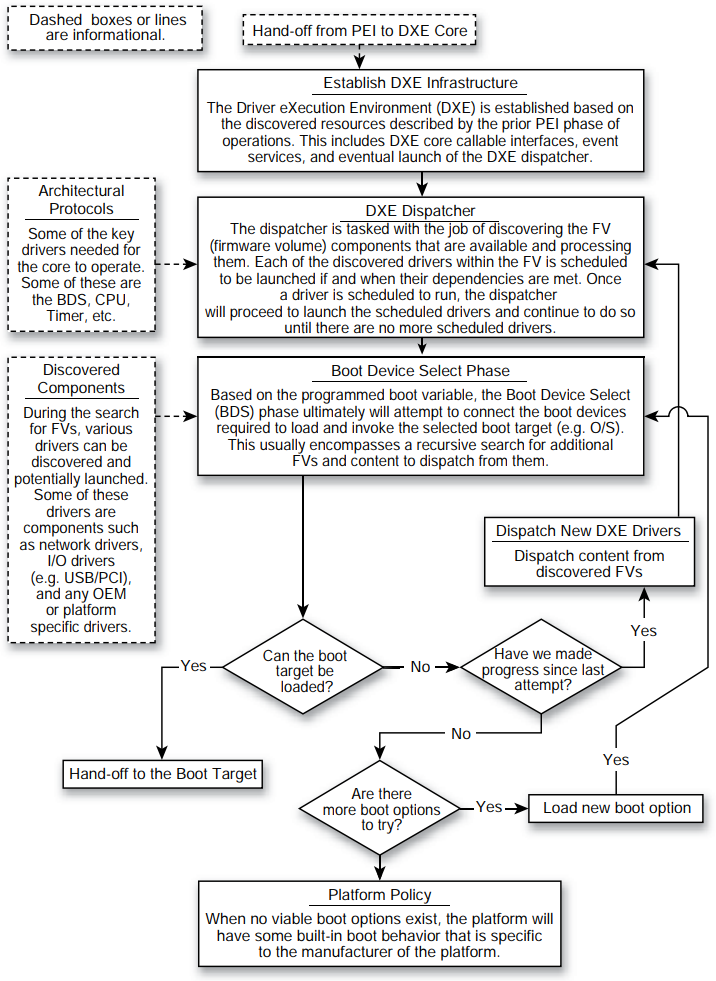
\includegraphics[width=\linewidth]{design/dxe-phase}
	\caption{DXE Phase}\label{fig:dxe-phase}
\end{figure}

DXE phase includes three major components as shown in Figure \ref{fig:dxe-components} which work among each other with the aim to initialize the platform and serve the services needed for performing OS boot.


\begin{figure}[!htbp]
	\centering
	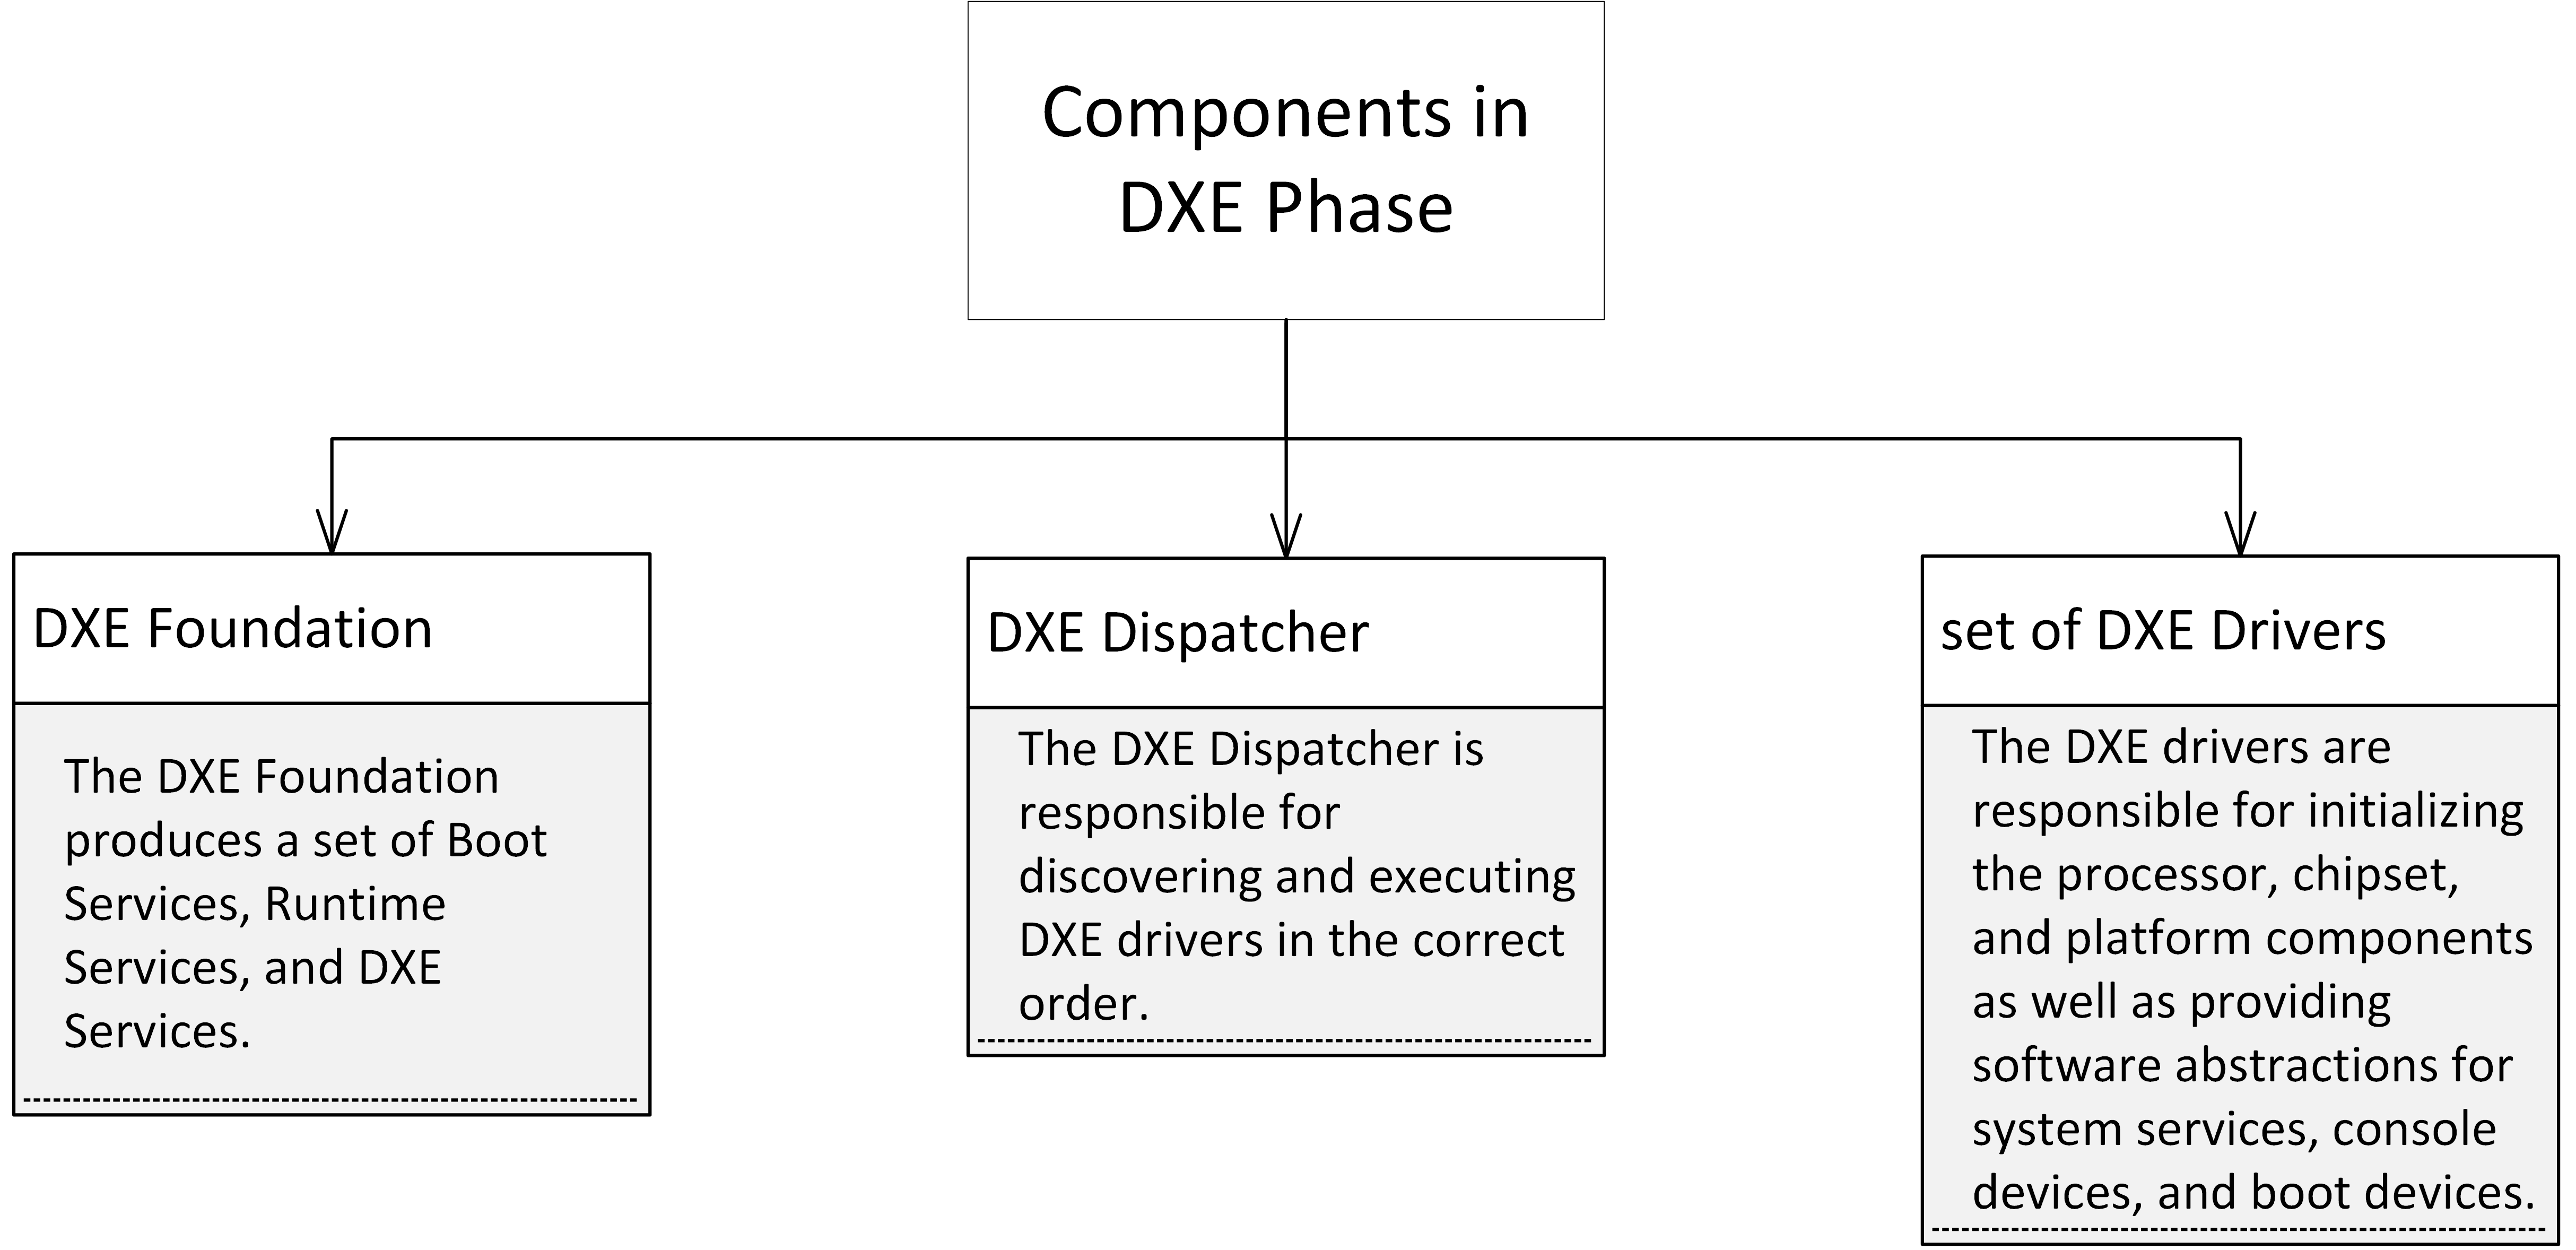
\includegraphics[width=\linewidth]{design/dxe-components}
	\caption{Components of DXE Phase}\label{fig:dxe-components}
\end{figure}


\subsection{Boot Device Selection (\gls{bds})}
The \say{BDS Architectural Protocol} has part of implementation of the Boot Device Selection (BDS) phase. After evaluation of all the dependencies of the DXE drivers along with their satisfied dependencies are loaded and execution is completed by the DXE Dispatcher, the DXE Foundation transfer the control flow to the BDS Architectural Protocol.

The \say{BDS Phase} held liable for:
\begin{itemize}
	\item Initialize the console devices
	\item Load the device drivers
	\item Attempt to load and execute the boot selection
\end{itemize}

\subsection{Transient System Load (TSL) and Runtime (RT)}
Primarily the OS vendor provides boot loader known as The \say{Transient System Load (TSL)}. TSL and Runtime Services (RT) phases may allow access to persistent content, via UEFI drivers and applications. Drivers in this category include PCI Option ROMs.

\subsection{After Life (AL)}
The After Life (AL) phase contains the persistent UEFI drivers used to store the state of the system during the OS systematically shutdown, sleep, hibernate or restart processes.
